%%%%%%%%%%%%%%%%%%%%%%%%%%%%%%%%%%%%%%%%%%%%%%%%%%%%%%%%%%%%%%%%%%%%%%%%%%%%%%%%
%2345678901234567890123456789012345678901234567890123456789012345678901234567890
%        1         2         3         4         5         6         7         8

\documentclass[letterpaper, 10 pt, conference]{ieeeconf}  % Comment this line out
                                                          % if you need a4paper
%\documentclass[a4paper, 10pt, conference]{ieeeconf}      % Use this line for a4
                                                          % paper

\IEEEoverridecommandlockouts                              % This command is only
                                                          % needed if you want to
                                                          % use the \thanks command
\overrideIEEEmargins
% See the \addtolength command later in the file to balance the column lengths
% on the last page of the document



% The following packages can be found on http:\\www.ctan.org
\usepackage{graphics} % for pdf, bitmapped graphics files
\usepackage{epsfig} % for postscript graphics files
\usepackage{mathptmx} % assumes new font selection scheme installed
\usepackage{times} % assumes new font selection scheme installed
\usepackage{amsmath} % assumes amsmath package installed
\usepackage{amssymb}  % assumes amsmath package installed
\usepackage{smartdiagram}
\usepackage{tikz}
\usepackage{verbatim}




\title{\LARGE \bf
LightGBM: an Effective Decision Tree Gradient Boosting Method to Predict Customer Loyalty in the Finance Industry*
}

%\author{ \parbox{3 in}{\centering Huibert Kwakernaak*
%         \thanks{*Use the $\backslash$thanks command to put information here}\\
%         Faculty of Electrical Engineering, Mathematics and Computer Science\\
%         University of Twente\\
%         7500 AE Enschede, The Netherlands\\
%         {\tt\small h.kwakernaak@autsubmit.com}}
%         \hspace*{ 0.5 in}
%         \parbox{3 in}{ \centering Pradeep Misra**
%         \thanks{**The footnote marks may be inserted manually}\\
%        Department of Electrical Engineering \\
%         Wright State University\\
%         Dayton, OH 45435, USA\\
%         {\tt\small pmisra@cs.wright.edu}}
%}

\author{Marcos Roberto Machado$^{1}$, Salma Karray$^{1}$ % <-this % stops a space
\thanks{*Submitted to Prof. Dra. Salma Karray as a report/article suggestion. This text was elaborated based on a ML grad course presentation performed at The Fields Institute in April 2019.}% <-this % stops a space
\thanks{$^{1}$University of Ontario Institute of Technology}
%,
%        University of Twente, 7500 AE Enschede, The Netherlands
%        {\tt\small h.kwakernaak at papercept.net}}%
%\thanks{$^{2}$P. Misra is with the Department of Electrical Engineering, Wright State University,
%        Dayton, OH 45435, USA
%        {\tt\small p.misra at ieee.org}}%
}




\begin{document}



\maketitle
\thispagestyle{empty}
\pagestyle{empty}


%%%%%%%%%%%%%%%%%%%%%%%%%%%%%%%%%%%%%%%%%%%%%%%%%%%%%%%%%%%%%%%%%%%%%%%%%%%%%%%%
\begin{abstract}
xxxxxxxxxxxxxxxxxxxxxxxxxxxxxxxx.
\end{abstract}


%%%%%%%%%%%%%%%%%%%%%%%%%%%%%%%%%%%%%%%%%%%%%%%%%%%%%%%%%%%%%%%%%%%%%%%%%%%%%%%%
\section{INTRODUCTION}
In order to maximize profits, companies have invest their efforts in trying to retain customers, boosting customers satisfaction levels and as a consequence escalating their loyalty. The intensity of customers satisfaction is a key metric for a company's CRM (Customer Relationship Management) and as a consequence, loyalty can also measure and analyzed as well. Although customer satisfaction and loyalty are key mediators of profit, they cannot be taken as simple predictors of it. From a business standpoint, it is more important to identify and nurture relationships specifically with profitable customers (Kumar and Reinartz, 2012 \cite{Kumar2012}). In this context artificial intelligence can be use through the application of Machine Learning (ML) and Deep Learning (DL) models given the extraordinary amount of customer information to businesses.\\

ML and DL models can be apply within customer loyalty context from two different point of views. Firstly, it can be use to measure loyalty given customers information, and, secondly, it can be apply to improve the customer satisfaction by providing the right product or service in the right channel/place at the correct time. In both cases, ML/DL models would learn from previous customer interactions. So important it is be focus on customer satisfaction and loyalty that, according to Gerry Brown from IDC, 2017 \cite{IDC2017}, 65\% of the marketing executives surveyed pointed out that ''real-time personalized advertising insertions" and ''optimized message targeting" will convey a compelling value by 2020. Also, a research published by MIT and Google said that 50\% of businesses intend to apply ML for customers insights, and 48\% expect it to earn a competitive advantage. \\ 

Some customer loyalty researches had applied ML techniques (Serkan, 2016 \cite{Loyal2016}; Ajay et al. 2019 \cite{loyal2019} and Davies et al. 2018 \cite{loyal2018}). More general, other business metrics such as customer lifetime value (CLV), customer retention or customer churn were also explored using ML models and different applications were found at the literature (Jamalian and Foukerdi, 2018 \cite{Jamalian2018}, Jing and Xing-hua, 2008 \cite{Zhao2008}, Amin et al. 2017 \cite{Amin2018} and Amin et al. 2018 \cite{Amin2018}). Moreover, none of these applications studied customer loyalty for credit card customers using LightGBM model.\\

The aim of this study is to explore the application of LightGBM as a predictor for a customer loyalty score. The problem was motivated based in an online competition (Kaggle, \cite{Kaggle}), where a credit card company is looking for a ML model that would make possible to predict a customer loyalty score for each single Card ID (for each single card issued). Company is also requesting a RMSE (Root Mean Square Error) to be presented along to the loyalty score predicted. These type of problem is getting more and more common in the financial industry, where, with more customer data it is more important to anticipate customers needs in order to retain them, increasing their loyalty. LightGBM as applied as the main ML method, mainly based on its capacity to uses GPU and uses less memory, the possibility to get high speed and handle large size of data. Also, because it present better accuracy than other decision tree gradient boosting models such as XBoosting (Ke et al., 2017 \cite{LGBM}) and by reason of its application was not found at the CRM/Loyalty literature.

\section{LITERATURE REVIEW}
\subsection{Decision Tree Models}
Falar um pouco de como decision tree models funcionam. Fazer uma revisao de literatura rasa.

\subsection{Gradient Boosting Models}
Fazer uma revisao de literatura rasa de modelos de grad boosting.

\subsection{DTGB Models}
Fazer uma revisao de literatura mais completa de como esses modelos funcionam, em especial, DT and GB.

\subsubsection{LightGBM}
\subsubsection{XBoosting}

\section{METHODOLOGY}
\subsection{Datasets}

Elo is one of the largest payment brands in South America. Elo results from a partnership of three of the largest banks in Brazil: Banco do Brasil, Bradesco and CAIXA. Elo offers credit, debit, and prepaid cards. At the end of 2018, Elo had issued more than 50 million cards. Also, Elo credit card supports installments payments, which allows a customer to arrange payments for a period of time.\\

Elo has built partnerships with merchants in order to offer promotions or discounts to cardholders. They have built machine learning models to understand the most important aspects and preferences in their customers’ lifecycle, from food to shopping. They also had built machine learning models to attribute a loyalty score for cluster of customers (per segment), however so far none of them is specifically tailored for an individual or profile (Kaggle, 2018 \cite{Kaggle}). This is where the Kaggle competition and data made available comes in, the main objective is to develop algorithms to identify a customer loyalty score for each card identified at the datasets.\\

Different datasets were made available (Figure \ref{Fig_data}). The historical dataset has transaction information, features such as purchase date and amount, number of installments, city and state, also a merchant identification and a sub sector identification of the merchant where card was used. The merchant dataset has additional information with respect to the places where cards were used. Features such as merchant id group, average sales, average purchase, active month lags, city and state of the merchant location were available. New merchant  has same type of information that historical data frame has, however this set of data contains material info of merchants visited for the first time. Train dataset contains the first month of activation, the target (loyalty score) and other features. All five data sets also have anonymous information/features.\\

\begin{figure}[thpb]
\centering
\smartdiagramset{set color list={green!40,magenta!40,blue!50,teal!40,orange!40},uniform connection color=true}
\smartdiagram[descriptive diagram]{
  {Historical,{Up to 3 months of historical transactions for each card identified.}},
  {Merchant, {Additional information about all merchants.}},
  {New Merchant, Two months of data for each card identified containing all purchases from each card made at each merchant not visited in the historical data.},
  {Test, The test set - which contains different features from the historical data.},
  {Train, The training set in the same format of the test set dataset.}}
\caption{Five different datasets were made available from ELO, a credit card company. Dataset are briefly described, each dataframe has different set of infromations. Data was published at kaggle.com in 2018 \cite{Kaggle}}
\label{Fig_data}
\end{figure}


\subsection{Data Preparation}
Almost all ML algorithms cant not perform well with missing values. This was the very first thing treat at the Data Preprocessing Treatment (DPT), which is part of what we are calling Data Cleaning. At this stage, for all datasets missing values were replaced based on the following rule: if the number of missing observations were less than 5\% of the total of instances for that feature, those observations were drop, in the other case, the missing value was replaced by the mode of that feature. In addition, an analysis over possible outliers was performed. It is important to highlight that, mainly for the target, 1.1\% (2,207) observations were possible outliers, and given the relevance of the feature in the data, those values were marked, considering the inclusion of a dummy feature in order to identify those.\\

In a second stage of a DPT, categorical features were converted to numerical values in order to facilitate things later on at the pipeline process. Codes were attribute to different nominal observation and this standard was applied for all datasets. Then, feature engineering was performed. Firstly, all the datasets were unified/appended by the card identification, then more features were create based in the ones that the company made available. Feature transformers were applied in order to provide more data information to the models learn better and predict information with higher accuracy. At the fourth stage, a correlation analysis over the features was implemented. When correlation was higher than 90\% features (new features created or previous ones) were drooped from the datasets. Finally, at the end of these workflow, a pipeline was implemented in order to select possible models and techniques to be use to train the data and do predictions. A workflow process is presented at Figure \ref{workflow}, where the bottom to top Data Preprocessing Treatment (DPT) performed in this study is presented. \\


\begin{figure}[thpb]
\centering
\smartdiagramset{set color list={orange!40,teal!40,blue!50,magenta!40,green!40},uniform connection color=true}
\smartdiagram[priority descriptive diagram]{
  Data Cleaning,
  Handling Text and Categorical Attributes,
  Feature Engineering,
  Correlation Analysis,
  Pipe Line Planning}
\caption{Workflow from bottom to top of the Data Preprocessing Treatment (DPT) performed in the datasets in this study. All steps in this process was recommended by Geron, 2017 \cite{Geron} and it is usually performed in an end-to-end ML modelling project.}
\label{workflow}
\end{figure}  
  

\subsection{Model Training}
%This needs to be written
In order to perform predictions at the test set, the main parameters used at LightGBM training process were:

\begin{itemize}
\item Number of leaves: 31;
\item Minimum amount of data in a leaf: 30;
\item Objective: Regression;
\item Number of threads: 4;
\item Boosting: GBDT
\end{itemize}

Another important thing to mention with respect to the training process is that stratified random sampling method was used within this step. This is a method of sampling that was used to divide the data set that went through the DPT into smaller groups known as strata. In a stratified random sampling method, the strata are formed based on similar attributes or characteristics. Each new sample has the same size, in LightGBM it is necessary to define the number of strata, which in this study was define as 5 for all training performed. By using stratified random sampling method, it is possible to have a higher number of subsets to train the model and by doing this give the model the chance to obtain a better performance, because in this case, each new subset is used once as a test set while the others are used as a training ones, until all of those be a test set once. 

%	Highlight colors and text:
%	\colorbox{red}{Your first option of version control!!!}
%	\textcolor{blue}{The second option right away!!!!!!!!!}

\subsection{Evaluation Criteria}
Falar sobre o RMSE e justificar o porque dele foi utilizado.


\section{RESULTS}
This section aims to present how well LightGBM predict customer loyalty in the Financial sector, specifically for the case of Elo credit card company. RMSE is analyzed altering some of the parameters within the ML training algorithm such as learning rate and number of iterations, also a comparison between LightGBM and Xboosting is performed.

\subsection{RMSE vs Learning Rate}
Model was trained for different learning rates (0.001, 0.005, 0.01, 0.02, 0.03, 0.04, 0.05, 0.06, 0.07, 0.08, 0.09, 0.1) and the RMSE for the predicted loyalty score was calculated. Figure \ref{learning_rate} presents these results. It is possible to verify that when learning rate is approaching zero RMSE is not one of the best results. That happens because given a poor learning rate, when the algorithm is looking for the best solution, a local minimum is found and it is understand to be the global minimum. On the other hand, when learning rate is increasing, after a certain point (around learning rate equals to 0.04), the RMSE is stable as a not optimal solution as well. This behavior is given by the reason of when the algorithm is looking for the best solution, its path is big enough to attribute big steps and passes by the global minimum, finding a local minimum as well. For this specific study, a learning rate of 0.01 is just right offering the lower RMSE and as well best loyalty score prediction.

\begin{figure}[thpb]
\centering
%\framebox{\parbox{3in}{We suggest that you use a text box to insert a graphic (which is ideally a 300 dpi TIFF or EPS file, with all fonts embedded) because, in an document, this method is somewhat more stable than directly inserting a picture.
%}}
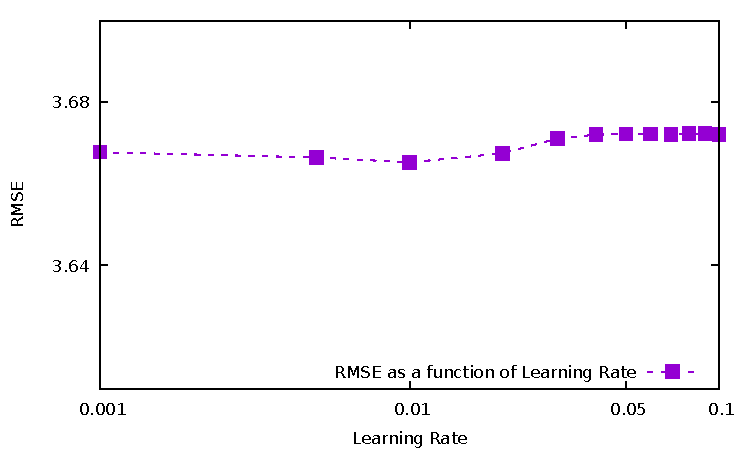
\includegraphics[scale=0.7]{Figures/learningrate_rmse_lgbm.pdf}
\caption{LightGBM results: RMSE as a function of learning rate.}
\label{learning_rate}
\end{figure}


\subsection{RMSE vs Number of Iterations}
For a fixed learning rate of 0.01, the learning rate which provides a better RMSE as presented previously, different number of iterations was input during model training. Mainly because LightGBM has a Decision Tree model growing in its code, it is important to verify how the RMSE would behave for different number of iterations, mainly because in a decision tree model depending on the number of iterations the model will ended it up with a different tree and as a consequence a different prediction. In this setting, different number of iterations were considered and RMSE measured, results are presented in Figure \ref{number_iterations}. \\

Graphic in Figure \ref{number_iterations} shows that for a small number of iterations the model does not have time enough to learn and find best solution and as a consequence a higher RMSE is observed. As the number of iterations increase, the RMSE decrease, up to a certain point where it does not matter how much more the number of iterations increase the RMSE will not present a significant change, it will just increase the processing time. Therefore, it is plausible to choose between 900-1000 iterations in this study and guarantee a the RMSE of the series.

\begin{figure}[thpb]
\centering
%\framebox{\parbox{3in}{We suggest that you use a text box to insert a graphic (which is ideally a 300 dpi TIFF or EPS file, with all fonts embedded) because, in an document, this method is somewhat more stable than directly inserting a picture.
%}}
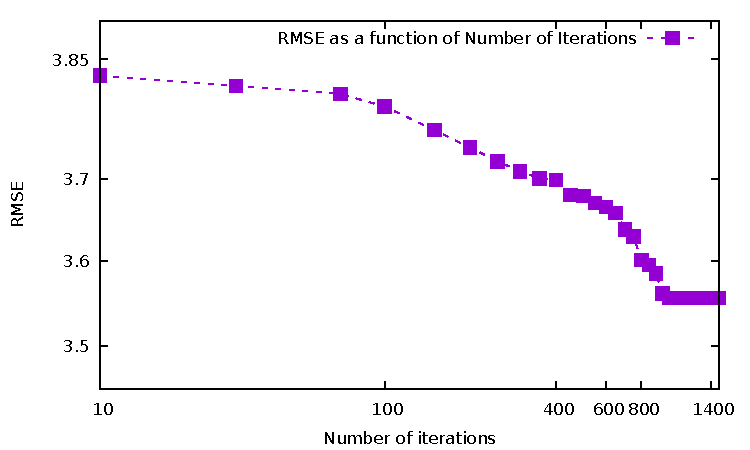
\includegraphics[scale=0.7]{Figures/numinteractions_rmse_lgbm.pdf}
\caption{LightGBM results: RMSE as a function of number of iterations.}
\label{number_iterations}
\end{figure}


\subsection{Training Time}
Another important thing to decide, from the point of view of a prediction model like the one explore in this study is based on a trade-off: time versus accuracy. The number of iterations was fixed at 1000 and output measures such as time and RMSE was calculated (Figure \ref{time}). It is possible to observe that for small learning rate time is between the highest in the interval and the RMSE is not optimal, and as the learning rate increase the processing time decrease, however the RMSE does not present a significant absolute difference in its value. Therefore, depending on the application CRM will have to decide what is the primarily focus - time or accuracy.

\begin{figure}[thpb]
\centering
%\framebox{\parbox{3in}{We suggest that you use a text box to insert a graphic (which is ideally a 300 dpi TIFF or EPS file, with all fonts embedded) because, in an document, this method is somewhat more stable than directly inserting a picture.
%}}
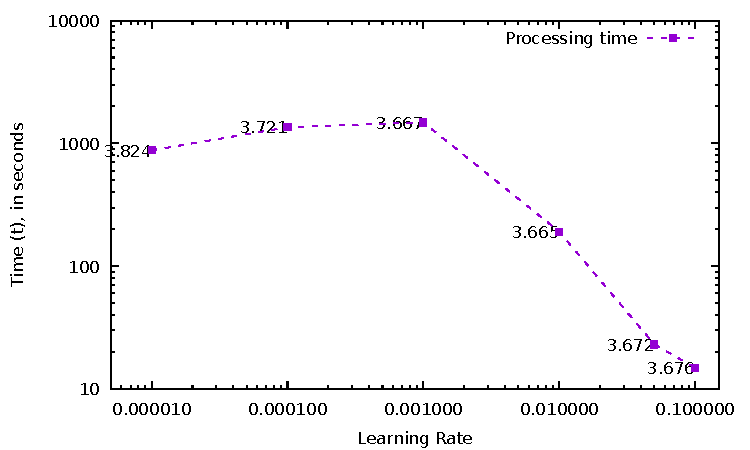
\includegraphics[scale=0.7]{Figures/time.pdf}
\caption{LightGBM results: Time and RMSE as a function of learning rate. RMSE is presented as a label for each point at the dotted line.}
\label{time}
\end{figure}


\subsection{Feature Importance}
Before perform model training, we ended up with more than 230 features. Feature importance in predicting customer loyalty in this study is given through the LightGBM model. Importance of each feature is calculated based on how many times a feature was used to slip information (was used as a node) during the tree growing in the modelling process. Figure \ref{feature_importance} presents the top 8 most important features and the least important to predict customer loyalty in this study, feature importance measure and standard deviation are presented. From approximately 200 features, only those are presented because they do not change when number of iterations or learning rate were altered. It is possible to observe that Month lag Mean, which is the average of months that a card identified was not used is the feature most used to split data in the decision tree process and the Month lag Minimum was the least one. Standard deviation slightly decrease as the feature importance decreases.

\begin{figure}[thpb]
\centering
%\framebox{\parbox{3in}{We suggest that you use a text box to insert a graphic (which is ideally a 300 dpi TIFF or EPS file, with all fonts embedded) because, in an document, this method is somewhat more stable than directly inserting a picture.
%}}
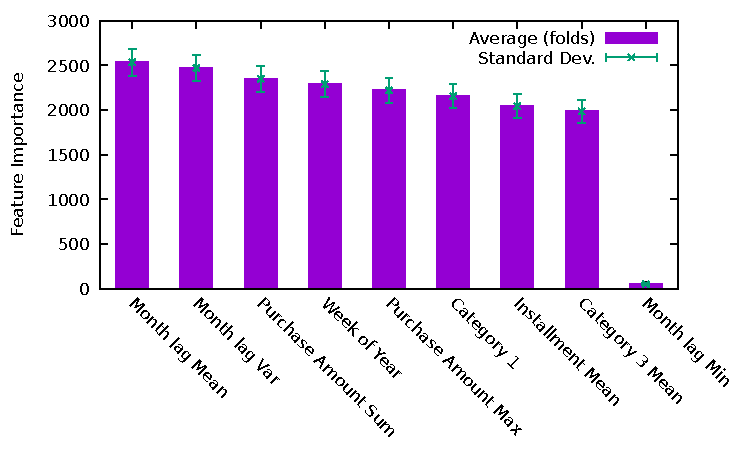
\includegraphics[scale=0.7]{Figures/Feature.pdf}
\caption{LightGBM results: Feature Importance.}
\label{feature_importance}
\end{figure}

\subsection{LightGBM vs XBoosting}
LightGBM and XBoosting are based on Decision Tree and Gradient Boosting (DTGB) techniques. However, based on the Ke et al., 2017 \cite{LGBM} affirmation that statement that LightGBM performs better than Xboosting as a DTGB combined model, this section aims to test this hypothesis. Same set of parameters were set up for both scenarios, information such as learning rate and number of iterations were fixed and RMSE was measured for both cases and are presented in Figure \ref{Xboosting}. It is possible to verify that, for this study, LightGBM perform better than XBoosting for all interval of learning rate used. Therefore, it is plausible to affirm that LightGBM can also be used as a DTGB model in the financial sector to predict customer loyalty.

\begin{figure}[thpb]
\centering
%\framebox{\parbox{3in}{We suggest that you use a text box to insert a graphic (which is ideally a 300 dpi TIFF or EPS file, with all fonts embedded) because, in an document, this method is somewhat more stable than directly inserting a picture.
%}}
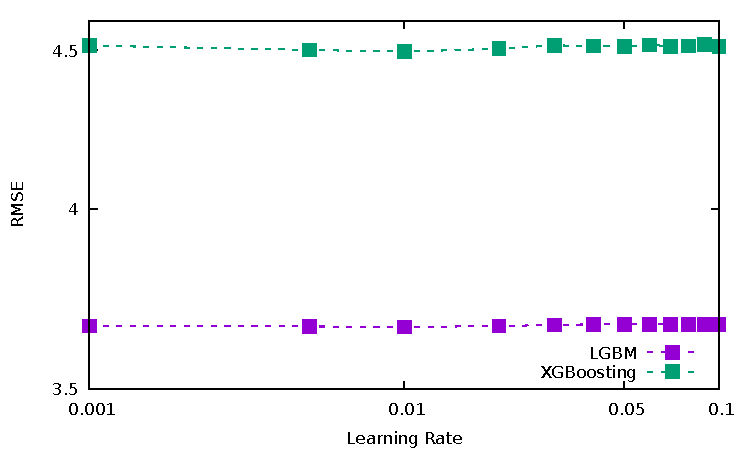
\includegraphics[scale=0.7]{Figures/learningrate_rmse_lgbm2.pdf}
\caption{LightGBM vs XBoosting: RMSE for customer loyalty prediction.}
\label{Xboosting}
\end{figure}



\section{CONCLUSION}
Olhar pra conclusao do artigo do hendrick pra ter uma ideia da ordem e do que escrever.


\addtolength{\textheight}{-12cm}   % This command serves to balance the column lengths
                                  % on the last page of the document manually. It shortens
                                  % the textheight of the last page by a suitable amount.
                                  % This command does not take effect until the next page
                                  % so it should come on the page before the last. Make
                                  % sure that you do not shorten the textheight too much.

%%%%%%%%%%%%%%%%%%%%%%%%%%%%%%%%%%%%%%%%%%%%%%%%%%%%%%%%%%%%%%%%%%%%%%%%%%%%%%%%



%%%%%%%%%%%%%%%%%%%%%%%%%%%%%%%%%%%%%%%%%%%%%%%%%%%%%%%%%%%%%%%%%%%%%%%%%%%%%%%%



%%%%%%%%%%%%%%%%%%%%%%%%%%%%%%%%%%%%%%%%%%%%%%%%%%%%%%%%%%%%%%%%%%%%%%%%%%%%%%%%


%%%%%%%%%%%%%%%%%%%%%%%%%%%%%%%%%%%%%%%%%%%%%%%%%%%%%%%%%%%%%%%%%%%%%%%%%%%%%%%%

\bibliographystyle{IEEEtran}
\bibliography{ref.bib}


\end{document}
